\documentclass[12pt,a4paper]{report}
\setlength\textwidth{145mm}
 \setlength\topmargin{0mm}
 \setlength\headsep{0mm}
 \setlength\headheight{0mm}
 
% Přepneme na českou sazbu
\usepackage[czech]{babel}
\usepackage[IL2]{fontenc}
\usepackage{graphicx} 

%% Použité kódování znaků: obvykle latin2, cp1250 nebo utf8:
\usepackage[utf8]{inputenc}
\begin{document}


\section{Triviální versus Cache-oblivious implementace}
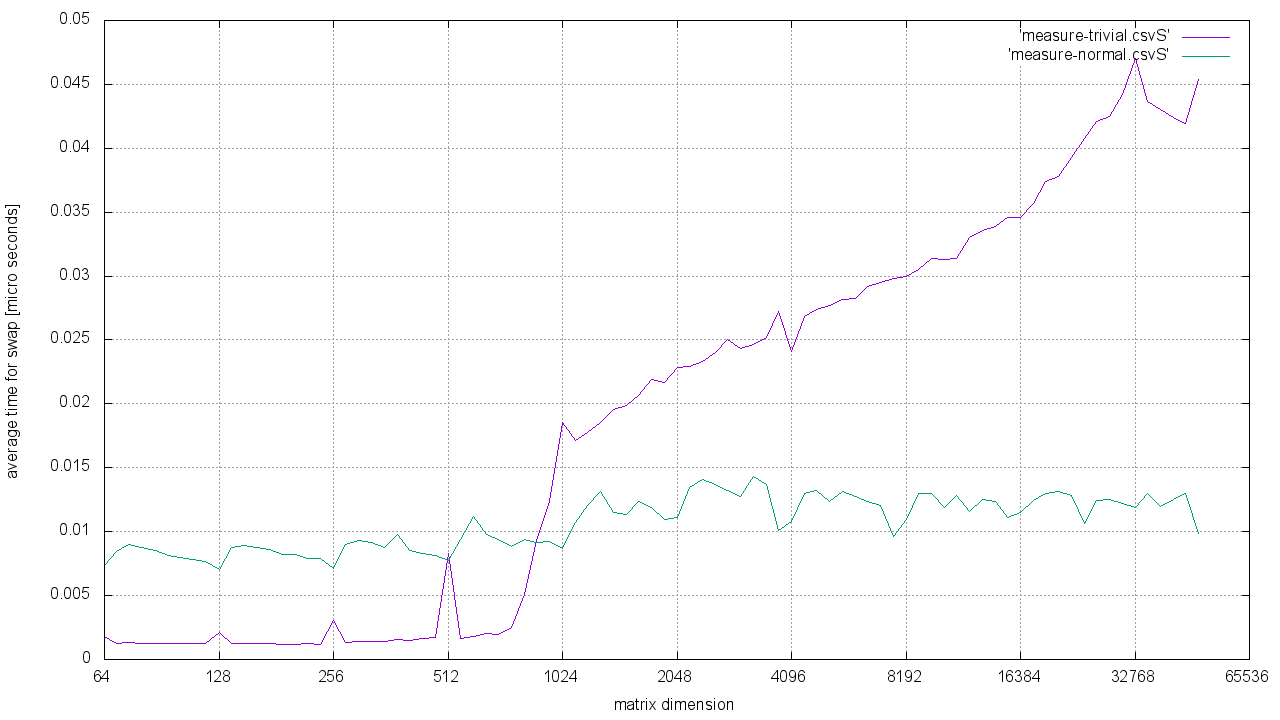
\includegraphics[width=\textwidth]{./tests/graph1.png}

Pro měření bylo použito až 10 GB paměti RAM.
Použitý počítač je osazen procesorem intel i7-920 @2.66 GHz
s 64-bitovými instrukecemi AMD64 a následujícími parametry cache:
\begin{itemize}
	\item L1 cache -- 32 kB,
	\item L2 cache -- 256 kB,
	\item L3 cache -- 8 MB.
\end{itemize}

Z grafu vidíme, že triviální implementace je o dost pomalejší.
Zároveň vidíme, že pro větší matice je vždy toto zpomalení větší.
V následujících bodech dochází u triviální implementace, ke zrychlení
růstu, zatímco u cache-oblivious algoritmu tato změna není pozorována.
\begin{itemize}
\item 850 MB  -- N=15000
\item 4,56 GB -- N=35000
\item 7,54 GB -- N=45000
\end{itemize}

Zvláštní je propad cache-oblivious algoritmu v posledním měřeném bodě, nejsem schopný
odhadovat, čím je způsoben.

\section{Simulace cache-oblivious algoritmu na ideální cache}
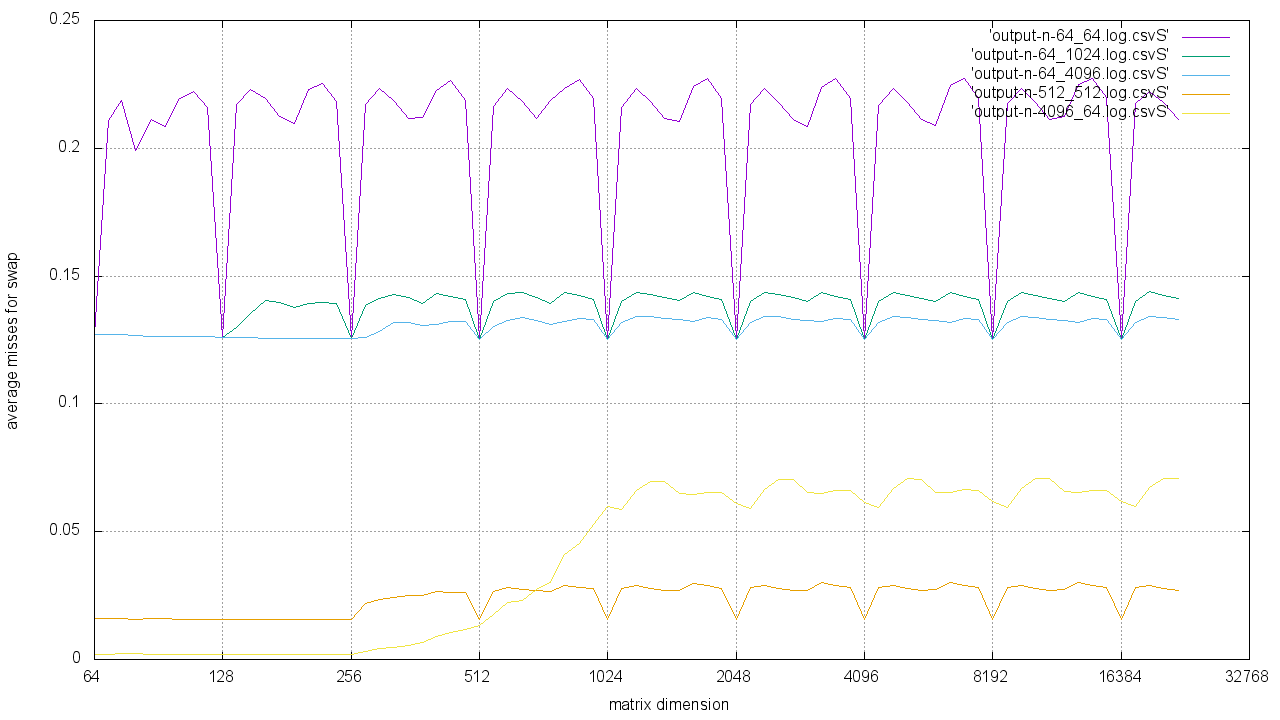
\includegraphics[width=\textwidth]{./tests/graph2.png}

Simulace jsme opět prováděly na stejných datech, jako při měření 
na počítači, nicměně pouze do maximalní velikosti matice 2 GB.
Předchozí graf znázorňuje závislost missů cache na počtu přístupů cache-oblivious algoritmu.

Vidíme, že vítězem byla cache s největší kapacitou, konkrétně cache s velikostí bloku 512 B
a počtem bloků 512. Zvýšení velikosti bloků na úkor jejich počtu (4096,64) vedlo k o něco horším výsledkům.
Naopak snížení velikosti bloků ve prospěch počtu bloků (64, 4096) vedlo opět ke zpomalení. 
Dále už je pořadí podle celkove velikosti cache. Vidíme tak, že je třeba volit vyvážený poměr
velikosti bloků a jejich počtu, aby cache fungovala co nejlépe.

Opět mi nejsou jasné pravidelné propady doby, které se vyskytují u všech typů cache. Nicméně
nejvíce jsou pozorovány u cache s nejmenší kapacitou.

\section{Simulace triviální verze algoritmu na ideální cache}
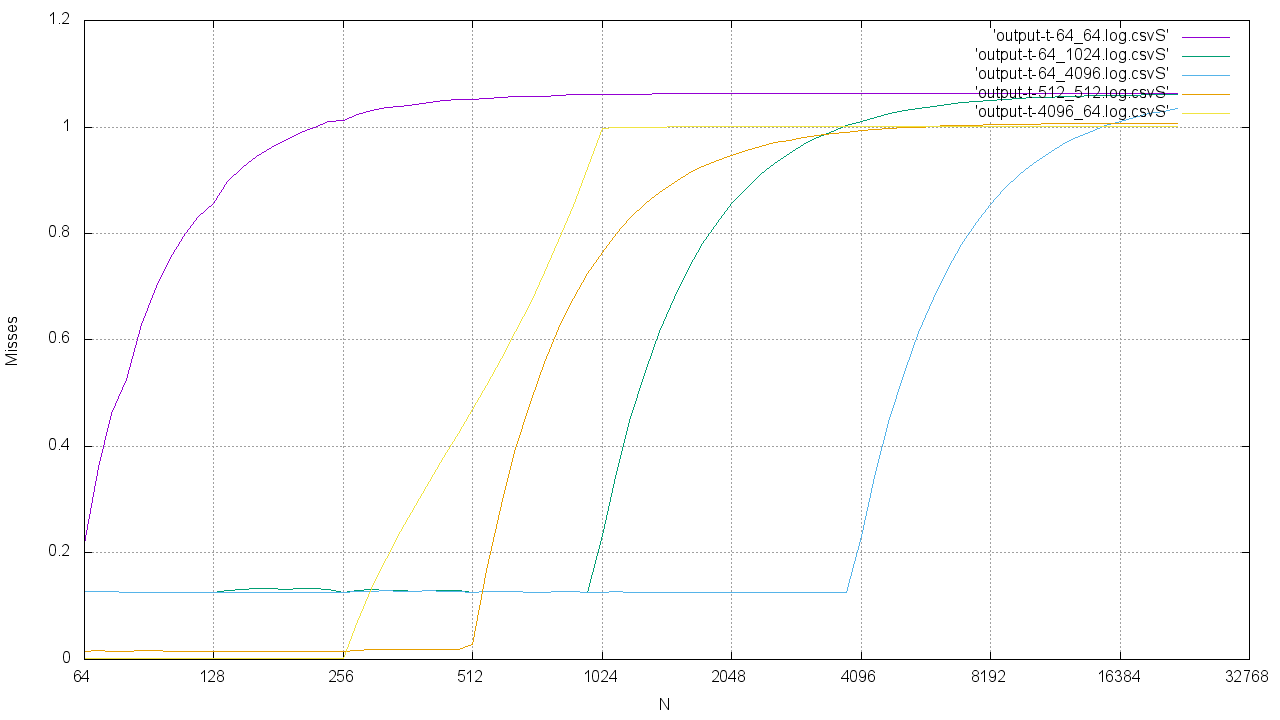
\includegraphics[width=\textwidth]{./tests/graph3.png}

Pro triviální verzi vidíme, že má řádově více cache missů. Také vidíme,
že nám nepomůže žádná verze cache, všechny jsou pro triviální verzi stejně špatné.



PS: možná by bylo dobré přiště někde napsat, že zadaní bylo modifikováno. 
(třeba bych pak úkol stihl odevzdat v časovém limitu, kdyz bych nemusel na rychlo provádět další testy...)
  
\end{document}
